% Graphic for TeX using PGF
% Title: /home/jnicolaschc/GitHub/Teoría de Telecominicaciones I /ttl1_trabajo3/Documentos/desarrollo/codigofuente/pgf/ventanasInicial.dia
% Creator: Dia v0.97+git
% CreationDate: Fri Aug 20 23:11:49 2021
% For: jnicolaschc
% \usepackage{tikz}
% The following commands are not supported in PSTricks at present
% We define them conditionally, so when they are implemented,
% this pgf file will use them.
\begin{figure}[H]
	\centering
	\ifx\du\undefined
		\newlength{\du}
	\fi
	\setlength{\du}{15\unitlength}
	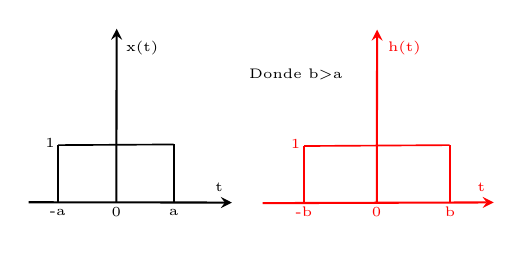
\begin{tikzpicture}[scale = 0.7]
		\pgftransformxscale{1.000000}
		\pgftransformyscale{-1.000000}
		\definecolor{dialinecolor}{rgb}{0.000000, 0.000000, 0.000000}
		\pgfsetstrokecolor{dialinecolor}
		\pgfsetstrokeopacity{1.000000}
		\definecolor{diafillcolor}{rgb}{1.000000, 1.000000, 1.000000}
		\pgfsetfillcolor{diafillcolor}
		\pgfsetfillopacity{1.000000}
		\pgfsetlinewidth{0.050000\du}
		\pgfsetdash{}{0pt}
		\pgfsetbuttcap
		{
			\definecolor{diafillcolor}{rgb}{0.000000, 0.000000, 0.000000}
			\pgfsetfillcolor{diafillcolor}
			\pgfsetfillopacity{1.000000}
			% was here!!!
			\pgfsetarrowsend{stealth}
			\definecolor{dialinecolor}{rgb}{0.000000, 0.000000, 0.000000}
			\pgfsetstrokecolor{dialinecolor}
			\pgfsetstrokeopacity{1.000000}
			\draw (33.016000\du,15.011800\du)--(33.027500\du,9.028390\du);
		}
		\pgfsetlinewidth{0.050000\du}
		\pgfsetdash{}{0pt}
		\pgfsetbuttcap
		{
			\definecolor{diafillcolor}{rgb}{0.000000, 0.000000, 0.000000}
			\pgfsetfillcolor{diafillcolor}
			\pgfsetfillopacity{1.000000}
			% was here!!!
			\pgfsetarrowsend{stealth}
			\definecolor{dialinecolor}{rgb}{0.000000, 0.000000, 0.000000}
			\pgfsetstrokecolor{dialinecolor}
			\pgfsetstrokeopacity{1.000000}
			\draw (30.001400\du,15.000400\du)--(36.993500\du,15.011800\du);
		}
		\pgfsetlinewidth{0.040000\du}
		\pgfsetdash{}{0pt}
		\pgfsetbuttcap
		{
			\definecolor{diafillcolor}{rgb}{0.000000, 0.000000, 0.000000}
			\pgfsetfillcolor{diafillcolor}
			\pgfsetfillopacity{1.000000}
			% was here!!!
			\definecolor{dialinecolor}{rgb}{0.000000, 0.000000, 0.000000}
			\pgfsetstrokecolor{dialinecolor}
			\pgfsetstrokeopacity{1.000000}
			\draw (31.010100\du,15.011800\du)--(31.010100\du,13.028800\du);
		}
		\pgfsetlinewidth{0.040000\du}
		\pgfsetdash{}{0pt}
		\pgfsetbuttcap
		{
			\definecolor{diafillcolor}{rgb}{0.000000, 0.000000, 0.000000}
			\pgfsetfillcolor{diafillcolor}
			\pgfsetfillopacity{1.000000}
			% was here!!!
			\definecolor{dialinecolor}{rgb}{0.000000, 0.000000, 0.000000}
			\pgfsetstrokecolor{dialinecolor}
			\pgfsetstrokeopacity{1.000000}
			\draw (34.993800\du,14.986000\du)--(34.993800\du,13.002900\du);
		}
		\pgfsetlinewidth{0.040000\du}
		\pgfsetdash{}{0pt}
		\pgfsetbuttcap
		{
			\definecolor{diafillcolor}{rgb}{0.000000, 0.000000, 0.000000}
			\pgfsetfillcolor{diafillcolor}
			\pgfsetfillopacity{1.000000}
			% was here!!!
			\definecolor{dialinecolor}{rgb}{0.000000, 0.000000, 0.000000}
			\pgfsetstrokecolor{dialinecolor}
			\pgfsetstrokeopacity{1.000000}
			\draw (31.010100\du,13.034500\du)--(34.987600\du,13.011600\du);
		}
		% setfont left to latex
		\definecolor{dialinecolor}{rgb}{0.000000, 0.000000, 0.000000}
		\pgfsetstrokecolor{dialinecolor}
		\pgfsetstrokeopacity{1.000000}
		\definecolor{diafillcolor}{rgb}{0.000000, 0.000000, 0.000000}
		\pgfsetfillcolor{diafillcolor}
		\pgfsetfillopacity{1.000000}
		\node[anchor=base,inner sep=0pt, outer sep=0pt,color=dialinecolor] at (30.998600\du,15.471197\du){\tiny -a};
		% setfont left to latex
		\definecolor{dialinecolor}{rgb}{0.000000, 0.000000, 0.000000}
		\pgfsetstrokecolor{dialinecolor}
		\pgfsetstrokeopacity{1.000000}
		\definecolor{diafillcolor}{rgb}{0.000000, 0.000000, 0.000000}
		\pgfsetfillcolor{diafillcolor}
		\pgfsetfillopacity{1.000000}
		\node[anchor=base,inner sep=0pt, outer sep=0pt,color=dialinecolor] at (34.989700\du,15.458054\du){\tiny a};
		% setfont left to latex
		\definecolor{dialinecolor}{rgb}{0.000000, 0.000000, 0.000000}
		\pgfsetstrokecolor{dialinecolor}
		\pgfsetstrokeopacity{1.000000}
		\definecolor{diafillcolor}{rgb}{0.000000, 0.000000, 0.000000}
		\pgfsetfillcolor{diafillcolor}
		\pgfsetfillopacity{1.000000}
		\node[anchor=base,inner sep=0pt, outer sep=0pt,color=dialinecolor] at (33.018100\du,15.474264\du){\tiny 0};
		% setfont left to latex
		\definecolor{dialinecolor}{rgb}{0.000000, 0.000000, 0.000000}
		\pgfsetstrokecolor{dialinecolor}
		\pgfsetstrokeopacity{1.000000}
		\definecolor{diafillcolor}{rgb}{0.000000, 0.000000, 0.000000}
		\pgfsetfillcolor{diafillcolor}
		\pgfsetfillopacity{1.000000}
		\node[anchor=base,inner sep=0pt, outer sep=0pt,color=dialinecolor] at (33.018100\du,15.897598\du){};
		% setfont left to latex
		\definecolor{dialinecolor}{rgb}{0.000000, 0.000000, 0.000000}
		\pgfsetstrokecolor{dialinecolor}
		\pgfsetstrokeopacity{1.000000}
		\definecolor{diafillcolor}{rgb}{0.000000, 0.000000, 0.000000}
		\pgfsetfillcolor{diafillcolor}
		\pgfsetfillopacity{1.000000}
		\node[anchor=base east,inner sep=0pt, outer sep=0pt,color=dialinecolor] at (30.894967\du,13.132469\du){\tiny 1};
		% setfont left to latex
		\definecolor{dialinecolor}{rgb}{0.000000, 0.000000, 0.000000}
		\pgfsetstrokecolor{dialinecolor}
		\pgfsetstrokeopacity{1.000000}
		\definecolor{diafillcolor}{rgb}{0.000000, 0.000000, 0.000000}
		\pgfsetfillcolor{diafillcolor}
		\pgfsetfillopacity{1.000000}
		\node[anchor=base,inner sep=0pt, outer sep=0pt,color=dialinecolor] at (36.555500\du,14.643575\du){\tiny t};
		% setfont left to latex
		\definecolor{dialinecolor}{rgb}{0.000000, 0.000000, 0.000000}
		\pgfsetstrokecolor{dialinecolor}
		\pgfsetstrokeopacity{1.000000}
		\definecolor{diafillcolor}{rgb}{0.000000, 0.000000, 0.000000}
		\pgfsetfillcolor{diafillcolor}
		\pgfsetfillopacity{1.000000}
		\node[anchor=base west,inner sep=0pt,outer sep=0pt,color=dialinecolor] at (33.350682\du,9.813504\du){\tiny x(t)};
		\pgfsetlinewidth{0.050000\du}
		\pgfsetdash{}{0pt}
		\pgfsetbuttcap
		{
			\definecolor{diafillcolor}{rgb}{1.000000, 0.000000, 0.000000}
			\pgfsetfillcolor{diafillcolor}
			\pgfsetfillopacity{1.000000}
			% was here!!!
			\pgfsetarrowsend{stealth}
			\definecolor{dialinecolor}{rgb}{1.000000, 0.000000, 0.000000}
			\pgfsetstrokecolor{dialinecolor}
			\pgfsetstrokeopacity{1.000000}
			\draw (41.979500\du,15.042600\du)--(41.991000\du,9.059170\du);
		}
		\pgfsetlinewidth{0.050000\du}
		\pgfsetdash{}{0pt}
		\pgfsetbuttcap
		{
			\definecolor{diafillcolor}{rgb}{1.000000, 0.000000, 0.000000}
			\pgfsetfillcolor{diafillcolor}
			\pgfsetfillopacity{1.000000}
			% was here!!!
			\pgfsetarrowsend{stealth}
			\definecolor{dialinecolor}{rgb}{1.000000, 0.000000, 0.000000}
			\pgfsetstrokecolor{dialinecolor}
			\pgfsetstrokeopacity{1.000000}
			\draw (38.047900\du,15.031100\du)--(46.003100\du,15.006100\du);
		}
		\pgfsetlinewidth{0.040000\du}
		\pgfsetdash{}{0pt}
		\pgfsetbuttcap
		{
			\definecolor{diafillcolor}{rgb}{1.000000, 0.000000, 0.000000}
			\pgfsetfillcolor{diafillcolor}
			\pgfsetfillopacity{1.000000}
			% was here!!!
			\definecolor{dialinecolor}{rgb}{1.000000, 0.000000, 0.000000}
			\pgfsetstrokecolor{dialinecolor}
			\pgfsetstrokeopacity{1.000000}
			\draw (39.480700\du,15.042600\du)--(39.480700\du,13.059600\du);
		}
		\pgfsetlinewidth{0.040000\du}
		\pgfsetdash{}{0pt}
		\pgfsetbuttcap
		{
			\definecolor{diafillcolor}{rgb}{1.000000, 0.000000, 0.000000}
			\pgfsetfillcolor{diafillcolor}
			\pgfsetfillopacity{1.000000}
			% was here!!!
			\definecolor{dialinecolor}{rgb}{1.000000, 0.000000, 0.000000}
			\pgfsetstrokecolor{dialinecolor}
			\pgfsetstrokeopacity{1.000000}
			\draw (44.496100\du,15.016700\du)--(44.496100\du,13.033700\du);
		}
		\pgfsetlinewidth{0.040000\du}
		\pgfsetdash{}{0pt}
		\pgfsetbuttcap
		{
			\definecolor{diafillcolor}{rgb}{1.000000, 0.000000, 0.000000}
			\pgfsetfillcolor{diafillcolor}
			\pgfsetfillopacity{1.000000}
			% was here!!!
			\definecolor{dialinecolor}{rgb}{1.000000, 0.000000, 0.000000}
			\pgfsetstrokecolor{dialinecolor}
			\pgfsetstrokeopacity{1.000000}
			\draw (39.480700\du,13.065300\du)--(44.490000\du,13.034500\du);
		}
		% setfont left to latex
		\definecolor{dialinecolor}{rgb}{1.000000, 0.000000, 0.000000}
		\pgfsetstrokecolor{dialinecolor}
		\pgfsetstrokeopacity{1.000000}
		\definecolor{diafillcolor}{rgb}{1.000000, 0.000000, 0.000000}
		\pgfsetfillcolor{diafillcolor}
		\pgfsetfillopacity{1.000000}
		\node[anchor=base,inner sep=0pt, outer sep=0pt,color=dialinecolor] at (39.469300\du,15.492359\du){\tiny -b};
		% setfont left to latex
		\definecolor{dialinecolor}{rgb}{1.000000, 0.000000, 0.000000}
		\pgfsetstrokecolor{dialinecolor}
		\pgfsetstrokeopacity{1.000000}
		\definecolor{diafillcolor}{rgb}{1.000000, 0.000000, 0.000000}
		\pgfsetfillcolor{diafillcolor}
		\pgfsetfillopacity{1.000000}
		\node[anchor=base,inner sep=0pt, outer sep=0pt,color=dialinecolor] at (44.503400\du,15.492359\du){\tiny b};
		% setfont left to latex
		\definecolor{dialinecolor}{rgb}{1.000000, 0.000000, 0.000000}
		\pgfsetstrokecolor{dialinecolor}
		\pgfsetstrokeopacity{1.000000}
		\definecolor{diafillcolor}{rgb}{1.000000, 0.000000, 0.000000}
		\pgfsetfillcolor{diafillcolor}
		\pgfsetfillopacity{1.000000}
		\node[anchor=base,inner sep=0pt, outer sep=0pt,color=dialinecolor] at (41.970200\du,15.492359\du){\tiny 0};
		% setfont left to latex
		\definecolor{dialinecolor}{rgb}{1.000000, 0.000000, 0.000000}
		\pgfsetstrokecolor{dialinecolor}
		\pgfsetstrokeopacity{1.000000}
		\definecolor{diafillcolor}{rgb}{1.000000, 0.000000, 0.000000}
		\pgfsetfillcolor{diafillcolor}
		\pgfsetfillopacity{1.000000}
		\node[anchor=base,inner sep=0pt, outer sep=0pt,color=dialinecolor] at (41.970200\du,15.915692\du){};
		% setfont left to latex
		\definecolor{dialinecolor}{rgb}{1.000000, 0.000000, 0.000000}
		\pgfsetstrokecolor{dialinecolor}
		\pgfsetstrokeopacity{1.000000}
		\definecolor{diafillcolor}{rgb}{1.000000, 0.000000, 0.000000}
		\pgfsetfillcolor{diafillcolor}
		\pgfsetfillopacity{1.000000}
		\node[anchor=base east,inner sep=0pt, outer sep=0pt,color=dialinecolor] at (39.346290\du,13.134352\du){\tiny 1};
		% setfont left to latex
		\definecolor{dialinecolor}{rgb}{1.000000, 0.000000, 0.000000}
		\pgfsetstrokecolor{dialinecolor}
		\pgfsetstrokeopacity{1.000000}
		\definecolor{diafillcolor}{rgb}{1.000000, 0.000000, 0.000000}
		\pgfsetfillcolor{diafillcolor}
		\pgfsetfillopacity{1.000000}
		\node[anchor=base,inner sep=0pt, outer sep=0pt,color=dialinecolor] at (45.579922\du,14.613913\du){\tiny t};
		% setfont left to latex
		\definecolor{dialinecolor}{rgb}{1.000000, 0.000000, 0.000000}
		\pgfsetstrokecolor{dialinecolor}
		\pgfsetstrokeopacity{1.000000}
		\definecolor{diafillcolor}{rgb}{1.000000, 0.000000, 0.000000}
		\pgfsetfillcolor{diafillcolor}
		\pgfsetfillopacity{1.000000}
		\node[anchor=base west,inner sep=0pt,outer sep=0pt,color=dialinecolor] at (42.368392\du,9.805729\du){\tiny h(t)};
		% setfont left to latex
		\definecolor{dialinecolor}{rgb}{0.000000, 0.000000, 0.000000}
		\pgfsetstrokecolor{dialinecolor}
		\pgfsetstrokeopacity{1.000000}
		\definecolor{diafillcolor}{rgb}{0.000000, 0.000000, 0.000000}
		\pgfsetfillcolor{diafillcolor}
		\pgfsetfillopacity{1.000000}
		\node[anchor=base west,inner sep=0pt,outer sep=0pt,color=dialinecolor] at (37.589600\du,10.730600\du){\tiny Donde b>a};
	\end{tikzpicture}
	\vspace{-3mm}
	\caption{\scriptsize Señales involucradas para generar una función trapezoidal.}
	\label{fig:ventanasIniciales}
\end{figure}
